\documentclass[a4paper,14pt,href,draft]{article}

% Используем нестандартный размер шрифта
\usepackage{extsizes}

% Делаем отступ для первого параграфа
\usepackage{indentfirst}

% Для поддержки поиска по pdf документу
\usepackage{cmap}

% Поддержка кириллицы
\usepackage[T2A]{fontenc}
\usepackage[utf8]{inputenc}
\usepackage[english,russian]{babel}

% Поддержка списков
\usepackage{enumerate}

% Заменяем библиографию с квадратных скобок на точку
\makeatletter
\renewcommand{\@biblabel}[1]{#1.}
\makeatother

% Графический пакет
\usepackage[final]{graphicx}
\usepackage{epstopdf}
\usepackage{tikz}

% Математические шрифты AMS
\usepackage{amstext, amssymb, amsmath}

% В заголовках появляется точка, но при ссылке на них ее нет
\usepackage{misccorr}

% Поддержка гиперссылок
\usepackage{url}

% Задаем полуторный межстрочный интервал
\linespread{1.3}

% Задаем глубину оглавления
\setcounter{tocdepth}{2}

% Путь к изображениям, по умолчанию
\graphicspath{{images/}}

% Задаем отступ абзаца
\setlength{\parindent}{1.25cm}

\renewcommand{\labelenumi}{\arabic{enumi}.}% Меняем везде перечисления на цифра.цифра

% Меняем поля страницы
\usepackage{geometry}
\geometry{left=2.5cm}   % левое поле
\geometry{right=2.5cm}  % правое поле
\geometry{top=2.5cm}    % верхнее поле
\geometry{bottom=2.5cm} % нижнее поле


% Листинг
\usepackage[final]{listings}
\usepackage{color}
\usepackage{xcolor}

\usepackage{caption}
\DeclareCaptionFont{white}{\color{white}}
\DeclareCaptionFormat{listing}{\colorbox{gray}{\parbox{\textwidth}{#1#2#3}}}
\captionsetup[lstlisting]{format=listing,labelfont=white,textfont=white}

\renewcommand{\lstlistingname}{Листинг}

\lstset{
  caption=Листинг,
  basicstyle=\footnotesize\ttfamily,
  numbers=left,
  numberstyle=\color{gray}\tiny,
  numbersep=5pt,
  tabsize=2,
  extendedchars=false,
  xleftmargin=17pt,
  framexleftmargin=17pt,
  framexrightmargin=5pt,
  framexbottommargin=4pt,
  showstringspaces=false,
  keepspaces = true}

% С++
\def\CC{{C\nolinebreak[4]\hspace{-.05em}\raisebox{.4ex}{\tiny\bf ++}}}

\begin{document}


%%%
% Титульный лист
%%%
\thispagestyle{empty}
\begin{center}
Федеральное государственное автономное образовательное учреждение \\
высшего профессионального образования \\
\textsc{<<Южный Федеральный Университет>>}\\[1.0cm]

Факультет математики, механики и компьютерных наук\\[1.0cm]

Направление подготовки 010400 \\
<<Прикладная математика и информатика>>\\[3cm]

А. А. Тактаров \\[1.0cm]
\textsc{Реактивный фреймворк для организации мультиагентных распределенных вычислений}\\[1.0cm]

\textit{Магистерская диссертация}\\[2.0cm]

\begin{flushright}
    Научные руководители: \\
    ст. преп. В. Н. Брагилевский \\
    доц., к.ф.-м.н. В. А. Савельев \\[1.0cm]

    Рецензент: \\
    доц., к. ф.-м. н. С. А. Гуда
\end{flushright}

\vfill

  Ростов-на-Дону\\
  2014
\end{center}

\newpage
\tableofcontents

\newpage
\section*{Введение}
\addcontentsline{toc}{section}{Введение}

Стремительный рост возможностей технологий беспроводной передачи данных и широкое распространение мобильных и
встраиваемых устройств способствовали появлению концепции так называемого <<Интернета вещей>>
(англ. \textit{Internet of Things})~\cite{IoTWired}, которая заключается в объединении всех окружающих людей вещей в
огромную вычислительную сеть. Участниками (\textbf{агентами}) такой сети являются устройства, которые способны собирать
информацию о физической среде, обрабатывать ее и реагировать на изменение состояния других агентов и всей системы в целом.
Стабильное функционирование такой сети позволяет с огромной скоростью внедрять и использовать такие технологии, как
<<умные>> датчики~\cite{NestThermostat}, носимые устройства (англ. \textit{wearable devices}), а также системы
автоматизированного управления домом. Кроме того, становление <<Интернета вещей>> влечет за собой появление
принципиально новых потоков информации, тщательный анализ которых позволит улучшать существующие системы
здравоохранения, безопасности и контролировать состояние окружающей среды.

Создание подобного рода сети невозможно без наличия функционирующей инфраструктуры, которая бы позволила быстро
и эффективно интегрировать новые компоненты. Исходя из распределенной природы описываемой сети, сформулируем необходимые
для этого требования:

\begin{enumerate}
  \item Соблюдение принципа системности при разработке~\cite{SystemPrinciple}. Продукт должен быть представлен в виде
  целой системы компонентов, каждый из которых обладает определенной функцией. Такие компоненты автоматически становятся
  автономными участниками сети.

  \item Однородность среды. Компоненты сети должны иметь возможность взаимодействовать между собой посредством
  стандартизированных протоколов и схем. Задачи идентификации, обеспечения целостности, конфиденциальности передаваемых
  данных должны по возможности быть решены этими протоколами.

  \item Открытость используемых технологий. Применение как программных, так и аппаратных решений, которые имеют
  открытую документацию, лояльные  условия использования и одновременно поддерживаются разными разработчиками
  (обычно целым сообществом), позволяет в определенных случаях решить проблему интеграции компонентов и сократить разрыв
  между разработкой и запуском в производство. Кроме того, открытые платформы предоставляют широкие возможности для
  начинающих команд разработчиков, что является благоприятным для формирования рынка.
\end{enumerate}

В данной работе описан процесс реализации и интеграции муль\-тиагентной системы на примере задачи распределенной
печати фотографий. В рамках разработанной системы устройство, печатающее фотографию, рассматривается как автономный
агент, который обладает состоянием и способен принимать и исполнять задания. Принципы, сформулированные выше, были
использованы в качестве основополагающих на этапах проектирования и разработки данного продукта.

\newpage
\section*{Постановка задачи}
\addcontentsline{toc}{section}{Постановка задачи}
Целью работы является разработка и развертывание системы, позволяющей организовать моментальную печать фотографий
пользователей социальной сети Instagram, распределяя задания печати среди подключенных к системе агентов ---
\textbf{печатных станций}, в состав которых входит печатное устройство --- принтер.

\begin{figure}[htbp]
\begin{center}
  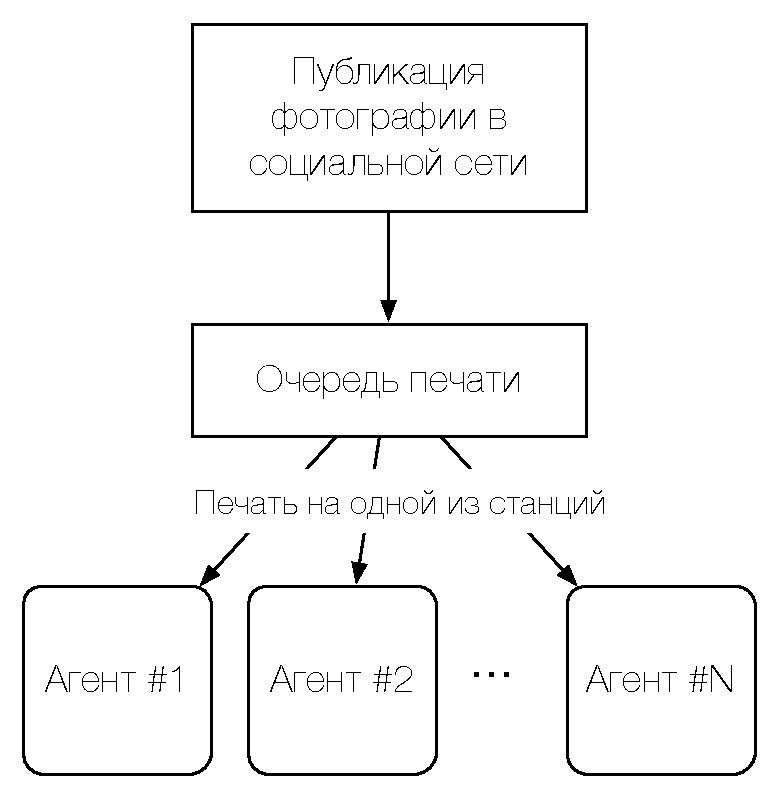
\includegraphics[scale=0.7]{print-schema.pdf}
    \caption{схема исполнения заданий печати}
    \label{fig:PrintSchema}
\end{center}
\end{figure}

Фотографии, которые публикуются пользователями социальной сети и удовлетворяют определенным условиям поиска
(содержат заранее известную метку --- \textit{хештег}), должны автоматически поступать в очередь печати системы.
Далее, исходная фотография, прошедшая определенную пост-обработку, печатается на одном из принтеров, входящих в
состав печатных станций (рис. \ref{fig:PrintSchema}). Информация о напечатанной фотографии сохраняется в системе для
отчетности. Функционирование такой системы позволяет организовать массовую печать фотографий во время проведения
мероприятий или для организации отложенной печати.

Сформулируем основные требования, предъявляемые к системе:
\begin{enumerate}
  \item Печатные станции могут быть физически отделены друг от друга, кроме того они могут находиться в разных
  сегментах сети. Необходим способ организации канала связи между агентами и контроль жизнеспособности этого канала.

  \item Необходим интерфейс управления печатными станциями и заданиями печати.

  \item Система должна иметь минимальный отклик и максимально быстро реагировать на изменение состояния компонентов.
  Изменение статуса задания печати (печать может завершиться успешно, а может закончиться неудачей в результате
  обрыва соединения) должно моментально отражаться в интерфейсе управления заданиями.
\end{enumerate}

Выделим последовательные этапы решения поставленной задачи:
\begin{enumerate}
  \item Проектирование архитектуры системы: разбиение системы на компоненты, выбор используемых при реализации
  каждого компонента технологий, построение схемы взаимодействия.

  \item Реализация компонентов системы, покрытие отдельных частей функциональными тестами.

  \item Решение задач интеграции и развертывании системы, настройка аппаратных средств.

  \item Опытное тестирование работы продукта.
\end{enumerate}

\newpage
\section{Архитектура системы}
В состав разработанного продукта входят три основных компонента: центральный сервер, агент печатной станции и
веб-приложение, предоставляющее интерфейс пользователя (рис. \ref{fig:Architecture}).

\begin{figure}[htbp]
\begin{center}
  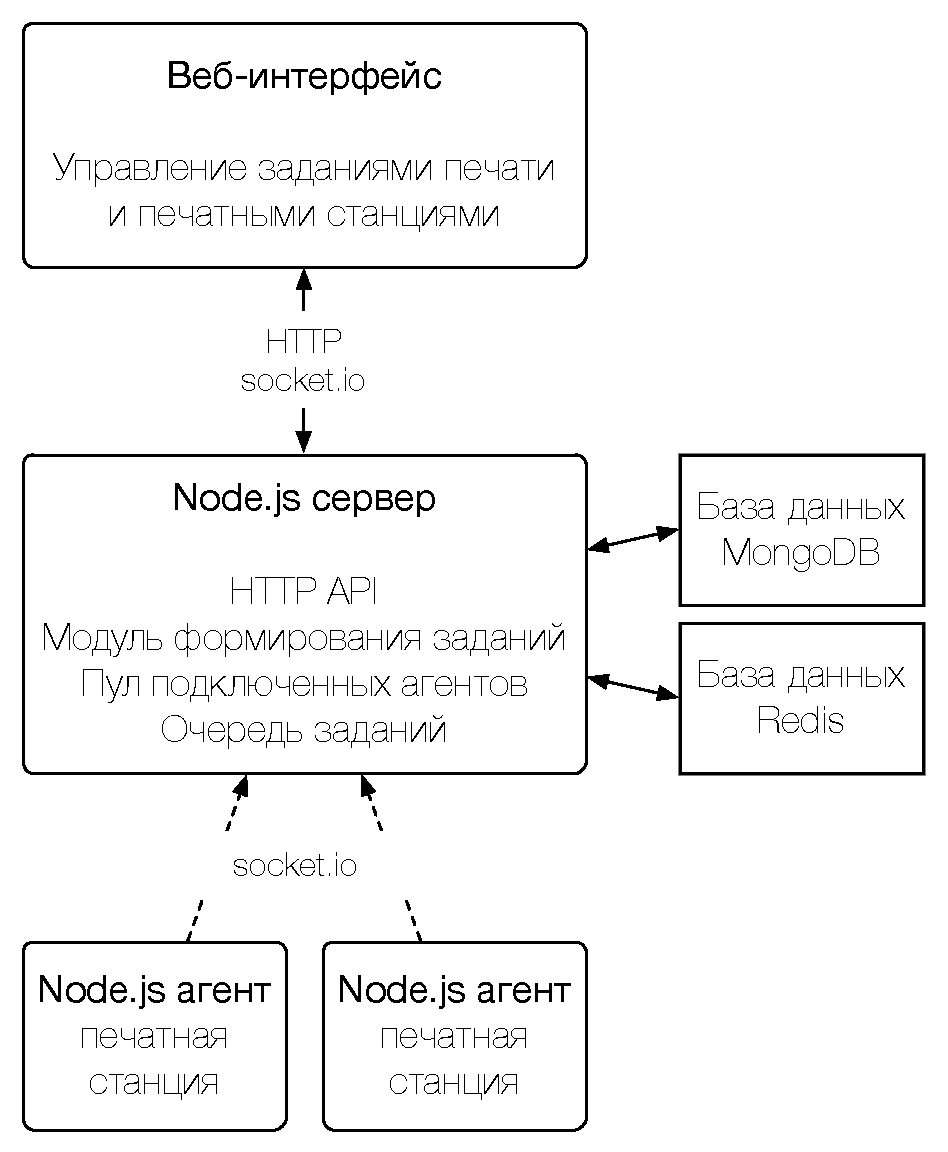
\includegraphics[scale=0.7]{architecture.pdf}
    \caption{архитектура системы}
    \label{fig:Architecture}
\end{center}
\end{figure}

Для хранения данных используются базы данных MongoDB и Redis, обращение к которым происходит через центральный сервер.
База данных MongoDB содержит информацию о зарегистрированных печатных станциях, администраторах системы, а также хранит
историю всех завершенных заданий печати. Средствами MongoDB реализована возможность гибкого поиска и
фильтрации данных~\cite{MongoDBBook}.

База данных Redis, являющаяся быстрым хранилищем типа <<ключ-значение>>, используется для организации очереди
заданий печати. Кроме того, благодаря возможности хранения данных в оперативной памяти данная база данных выступает в
роли хранилища сессий центрального веб-сервера.

\subsection{Центральный сервер}
Ядром системы является центральный сервер, в функции которого входит:

\begin{enumerate}
  \item Управление очередью печати. Модуль формирования заданий используется для поиска в социальной сети новых
  отмеченных для печати фотографий, которые помещаются в очередь печати. Распечатанные фотографий извлекаются из
  очереди, а ненапечатанные дополняются сообщением об ошибке для отчетности.

  \item Взаимодействие с подключенными по каналу связи агентами. Контроль качества канала связи и авторизация
  печатных станций.

  \item Предоставление прикладного программного интерфейса (API) на основе протокола HTTP.
\end{enumerate}

Данный компонент разработан на языке программирования \linebreak CoffeeScript~\cite{LittleCoffeeScript} и работает
на основе асинхронного серверного фреймворка Node.js. Решение по использованию данного инструментария было принято,
исходя из следующего:

\begin{enumerate}
  \item Платформа Node.js предоставляет широкие возможности по использованию низкоуровневых средств (работа с
  процессами, сокетами, бинарными данными и потоками ввода-вывода), предоставляя для этого удобный интерфейс на
  языке программирования JavaScript. Кроме того, все операции ввода вывода в Node.js являются асинхронными
  (то есть не блокируют исполнение программы), а контроль завершения происходит с помощью функций обратного вызова
  и событий. Обработка завершения асинхронных действий реализована в так называемой \textit{очереди обработки событий}
  (англ. \textit{event loop})~\cite{UnderstandingEvenLoop}, работающей на основе паттерна Проактор~\cite{BoostProactor}.

  \item Node.js позволяет разработчику использовать сторонние модули благодаря мощному пакетному менеджеру NPM.
  Простота публикации модулей и открытое сообщество разработчиков по всему миру способствовали развитию огромной
  инфраструктуры пакетов~\cite{NPMGrowth}. Таким образом, проектирование приложений заключается в разбиении на
  мелкие подзадачи, которые решаются с использованием готовых пакетов, что позволяет оптимизировать процесс разработки.

  \item Благодаря тому, что JavaScript является интерпретируемым языком, программы, написанные с использованием
  Node.js, являются кроссплатформенными. Существует поддержка операционных систем, совместимых с ARM-процессорами,
  что делает возможным запуск кода даже на встраиваемых устройствах.

  \item Язык программирования CoffeeScript является компилируемым в \newline JavaScript языком, расширяющим
  возможности последнего за счет полноценной поддержки объектно-ориентированной парадигмы и добавления
  <<синтаксического сахара>>. Синтаксические особенности языка делают возможным реализацию сложных паттернов
  проектирования, что является важным при разработке больших приложений~\cite{CoffeeScriptCookbook}.
\end{enumerate}

\subsection{Агент печатной станции}
В представленной системе компонентом, который исполняет задания печати, является агент печатной станции, подключенный к
центральному серверу. В задачи данного модуля входит:

\begin{enumerate}
  \item Принятие заданий печати от центрального сервера, представленных в виде изображения и метаинформации, в которую
  входят параметры печати и другие вспомогательные данные.

  \item Работа с локальной очередью печати подключенного принтера. Постановка на печать полученного изображения.

  \item Отправка отчета о статусе завершенного задания.
\end{enumerate}

Компонент разработан на языке программирования CoffeeScript и работает под управлением фреймворка Node.js. В отличие в
центрального сервера, который функционирует в режиме демона, подразумевается, что агент может быть запущен по требованию.
Более того, одновременно могут быть доступны несколько печатных станций, разнесенных физически и представленных в виде
отдельных экземпляров данного компонента.

\subsection{Организация канала связи между сервером и агентом}
При разработке мультиагентных систем особенно остро встает проблема организации канала связи, который обеспечивает
взаимодействие агентов с сервером, распределяющим задания. При проектировании таких систем становится очевидным, что
невозможно решить данную проблему, используя только возможности протокола TCP. Во-первых, следует учитывать, что
выход в сеть чаще всего всего происходит посредством NAT или межсетевого экрана, что ограничивает возможность
подключения (в таких условиях необходимо выделять центральный узел, чаще всего расположенный на выделенном сервере).
Во-вторых, должен быть способ поддержания длительных сессий между участниками (например, опция keepalive~\cite{Keepalive}
протокола TCP не реализована в старых версиях ядра Linux). Наконец, традиционная схема передачи данных не является
удобной при реализации реактивных систем, взаимодействие компонентов в которой обычно организовано в виде двунаправленной
передачи сообщений.

Для организации канала связи между сервером и печатной станцией в описываемой системе используется
свободно распространяемая библиотека socket.io~\cite{SocketIO}. Данная библиотека предоставляет следующие возможности:

\begin{enumerate}
  \item Организация дуплексного канала связи, который абстрагирован от среды запуска и транспорта. Возможно использование
  socket.io как в серверных и клиентских приложениях (написанных на Node.js), так и в веб-браузере. Для передачи данных
  могут использоваться технологии WebSockets или JSON Polling (периодический опрос сервера о наличии новых сообщений);
  переключение между этими транспортами является прозрачным.

  \item Автоматический контроль жизнеспособности канала. Это реализовано при помощи отправки серии служебных сообщений
  (heartbeats) от клиента к серверу и наоборот. В случае обрыва соединения происходит попытка повторного подключения,
  причем реализована стратегия экспоненциального увеличения интервала между неудачными попытками. Такое поведение доступно
  по умолчанию, и чаще всего процесс восстановления соединения скрыт от программиста.
\end{enumerate}

Узлы, использующие socket.io, обмениваются друг с другом сообщениями, которые сериализуются для отправки выбранным
транспортом. Сообщение можно представить в виде кортежа $(T, a_1, a_2, ..., a_N)$, где $T$ --- текстовый идентификатор
типа сообщения, $a_1, a_2, ..., a_N $ --- сериализованные параметры сообщения.

Библиотека socket.io предоставляет также возможность реализации удаленного вызова процедур (англ. RPC --- Remote
Procedure Call) благодаря механизму подтверждений (англ. \textit{acknowledgement}). Использование удаленного вызова
процедур на примере функции возведения в квадрат представлено в листинге \ref{lst:rpc}. Вызов удаленной функции происходит
как отправка сообщения, последним параметром которого является функция обратного вызова, которая будет исполнена, как только
удаленная сторона отправит ответ. Реализация удаленной функции также содержит параметр-функцию, которую необходимо вызвать
для возврата значения. Заметим, что этот параметр не является исходной функцией, которая была передана при отправке
сообщения. Ее вызов приводит к отправке подтверждающего сообщения, содержащего результат (рис. \ref{fig:RpcSchema}).

\begin{figure}[htbp]
\begin{center}
  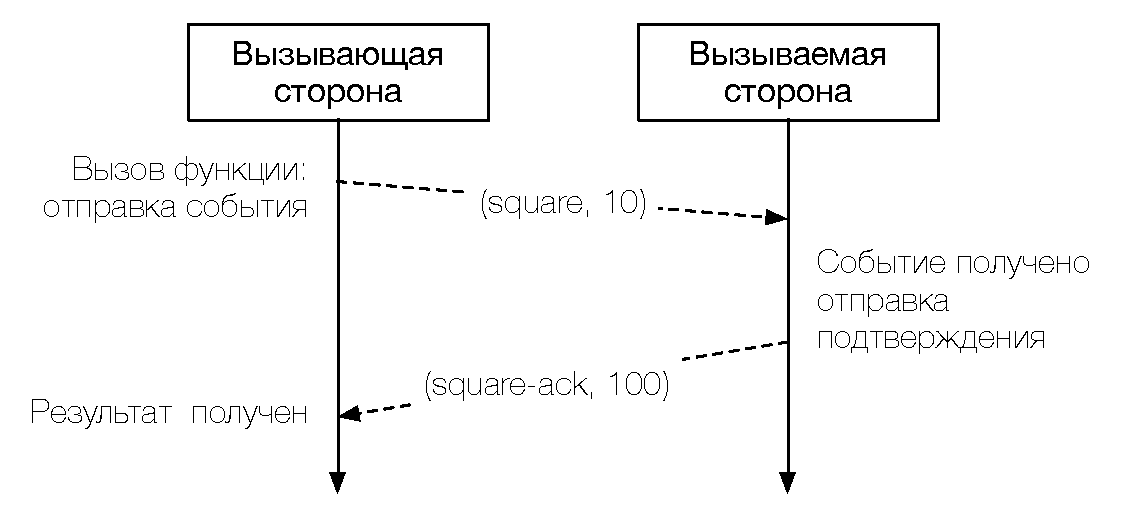
\includegraphics[scale=0.8]{rpc-schema.pdf}
    \caption{схема организации удаленного вызова процедур}
    \label{fig:RpcSchema}
\end{center}
\end{figure}

\begin{lstlisting}[caption=Удаленный вызов процедур в socket.io, label=lst:rpc]
  # RPC функция возведения числа в квадрат
  socket.on "square", (n, callback) ->
    # Вызов переданной функции выглядит как вызов
    # обычной функции
    callback n * n


  # Вызов RPC функции на клиенте выглядит как отправка сообщения.
  # Первый аргумент: тип сообщения
  # Второй аргумент: параметр сообщения
  # Третий аргумент это функция реакции на acknowledgement
  socket.emit "square", 10, (result) ->
    # Полученный результат: 100
    console.log result
\end{lstlisting}

При реализации агента печатной станции были использованы возможности удаленного вызова процедур для организации печати
заданий, полученных от центрального сервера.

\subsection{Веб-интерфейс}
Для удобного управления очередью печати и мониторинга состояния подключенных станций разработан интерфейс, представляющий
собой одностраничное веб-приложение, написанное на языке CoffeeScript. Взаимодействие интерфейса с центральным
 сервером происходит через его HTTP API с использованием парадигмы REST.

Веб-интерфейс построен с применением паттерна MVC (<<Model-View-Controller>> --- <<Модель-Вид-Контроллер>>)~\cite{ScalingIsomorphic},
реализо\-ван\-но\-го в клиентском веб-фреймворке Chaplin~\cite{ChaplinJS}. Особенность реализации заключается в том, что
подгрузка данных с сервера, их обработка, генерация представления этих данных и управление переходами между состояниями
веб-приложения полностью происходит на стороне веб-браузера, что позволяет снизить нагрузку на центральный сервер.
Кроме того, применение такого подхода означает, что собранное веб-приложение представимо в виде набора статичных файлов,
что делает возможным использование кеширования для ускорения загрузки страницы.

\newpage
\section{Особенности реализации}
В данной главе представлены детали реализации отдельных компонентов системы, в том числе касающиеся организации печати в рамках
печатной станции и очереди печати, здесь также описана модель хранимых в системе данных.
% Вообще, плохо сформулировано. Нужно дополнить.

\subsection{Организация печати}
Возможность совершения печати агентом реализована благодаря низкоуровневой работе с системным спулером печати и классу-обертке,
позволяющему получать уведомления в виде событий о статусе печати.

\subsubsection{Работа с системной очередью печати}
Взаимодействие с принтером происходит посредством постановки заданий в системную очередь печати (такая очередь называется
\textit{спулером} печати). В UNIX-подобных системах это осуществляется через CUPS (<<Common Unix Printing System>> ---
система печати в UNIX). Система CUPS была изначально спроектирована так, чтобы обеспечить поддержку печати в условиях
модели <<клиент-сервер>>, то есть допускает использование одного принтера сразу несколькими компьютерами в локальной сети.

Ключевым понятием в CUPS является \textbf{получатель} (англ. \textit{destina\-ti\-on}) печати. Получателем называется
доступный по сети принтер вместе с очередью печати. Фактически, любой локальный принтер в CUPS также воспринимается как
сетевой. Печать файла представляет собой подключение к определенному получателю и постановку файла в очередь.

Взаимодействие с CUPS происходит через API в виде библиотеки на языке C~\cite{CUPSAPI}. Для обеспечения возможности работы с CUPS
из кода агента (реализованного на Node.js) был разработан модуль-обертка на языке~\CC. Node.js предоставляет разработчикам
средства, позволяющие писать низкоуровневые модули, работа с которыми доступна в контексте исполнения JavaSript~\cite{NodeJSAddons}.

Задача модуля --- предоставление интерфейса для вызова функций CUPS посредством функций, доступных из JavaScript.
При этом следует учитывать, что переданные аргументы должны быть преобразованы из JavaScript-примитивов в типы данных,
которые поддерживает CUPS (например, экземпляр JavaScript класса \texttt{String} должен быть преобразован к C-строке).
Подобные трансформации в данном модуле реализованы благодаря функция и классам библиотеки V8, которая является движком,
используемым платформой Node.js.

Приведем список функций CUPS, поддержка которых была реализована:
\begin{description}
  \item[\texttt{cupsGetDests}] \hfill\\Возвращает список доступных получателей в локальной системе.
  \item[\texttt{cupsGetDefault}] \hfill\\Возвращает идентификатор получателя по умолчанию.
  \item[\texttt{cupsGetJobs}] \hfill\\Возвращает список всех заданий печати в очереди заданного получателя.
  \item[\texttt{cupsPrintFile}] \hfill\\Печать файла. Создает новое задание печати в очереди заданного получателя.
  \item[\texttt{cupsCancelJob}] \hfill\\Отменяет заданное задание печати.
\end{description}

Разработанный модуль опубликован в виде пакета в официальном репозитории NPM под названием \textbf{cupsidity}. Исходный
код модуля доступен в виде открытого репозитория и снабжен документацией~\cite{Cupsidity}.

\subsubsection{Высокоуровневый класс-обертка}
К сожалению, CUPS не предоставляет интерфейса, с помощью которого можно получать асинхронные события по изменению
статуса заданий печати, что противоречит принципу реактивности, указанному среди требований к разрабатываемой системе.
Единственным способом, позволяющим узнать, было ли завершено конкретное задание, является периодический вызов функции
\texttt{cupsGetJobs}.

\begin{figure}[htbp]
\begin{center}
  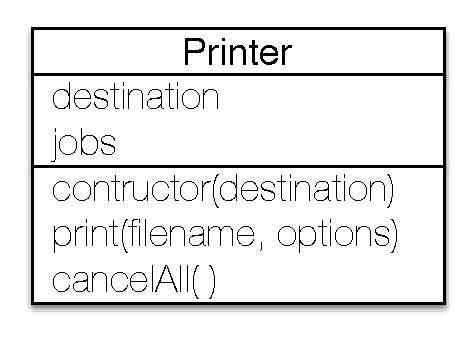
\includegraphics[scale=0.8]{printer-class.pdf}
    \caption{класс-обертка Printer}
    \label{fig:PrinterClass}
\end{center}
\end{figure}

Для предоставления асинхронного интерфейса для печати файлов был разработан класс-обертка \texttt{Printer} (рис.
\ref{fig:PrinterClass}). Конструктор класса принимает параметр \texttt{destination}, являющийся названием
принтера-получателя.


\begin{lstlisting}[caption=Печать файла с помощью класса \texttt{Printer}, label=lst:deferred]
  # Получаем доступ к принтеру
  printer = new Printer config.get "printer:name"

  # Печать файла
  printer.print(filename, config.get "printer:options")
  .then ->
    log.info "Job successfully printed"
    done null
  .fail (err) ->
    log.warn "Printing error: #{err}"
    done "Printing error"
\end{lstlisting}


Печать заданного файла осуществляется посредством вызова функции \texttt{print}, принимающей путь к печатаемому файлу и
необходимые параметры печати. Данная функция возвращает объект \texttt{Deferred}, который является одним из асинхронных
примитивов, входящих в состав библиотеки Q~\cite{QLibrary}. \texttt{Deferred} --- это представление завершенности отложенной
асинхронной операции, которая может находиться в следующих состояниях: ожидается (англ. \textit{pending}),
завершено (англ. \textit{resolved}), завершено с ошибкой (англ. \textit{rejected}). Пример вызова функции \texttt{print}
и обработка состояний объекта \texttt{Deferred} представлены в листинге \ref{lst:deferred}.

\begin{figure}[htbp]
\begin{center}
  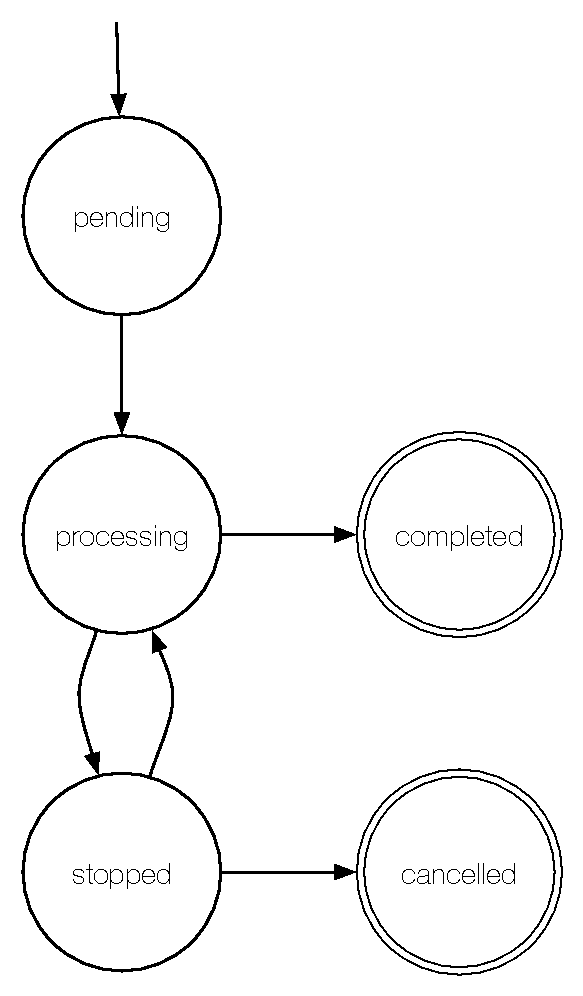
\includegraphics[scale=0.65]{state-machine.pdf}
    \caption{диаграмма состояний задания печати}
    \label{fig:StateMachine}
\end{center}
\end{figure}

Вызов функции \texttt{print} приводит к созданию задания печати, которое может находиться в следующих состояниях:
\begin{description}
  \item[\texttt{pending}] \hfill\\Задание находится в очереди и ждет обработки. Это начальное состояние задания.
  \item[\texttt{processing}] \hfill\\Задание исполняется (происходит печать).
  \item[\texttt{completed}] \hfill\\Задание завершено (файл напечатан). Это терминальное состояние, которое свидетельствует
  об успешном завершении задания.
  \item[\texttt{stopped}] \hfill\\Задание приостановлено. Причиной остановки могут быть проблемы, связанные с оборудованием и
  расходными материалами: закончилась бумаги или краска, связь с принтером прервалась и т.~д.
  \item[\texttt{cancelled}] \hfill\\Задание отменено. Терминальное состояние, свидетельствующее о том, что во время печати
  произошли ошибки.
\end{description}

Возможные переходы между описанными состояниями приведены на рис. \ref{fig:StateMachine}. Класс \texttt{Printer} содержит
приватную функцию \texttt{stateCheckRou\-ti\-ne}, которая вызывается с определенным интервалом времени и детектирует
переход между состояниями заданий печати, которые были назначены на заданный принтер. Переход задания в одно из терминальных
состояний означает завершение процесса печати и приводит к завершению соответствующего объекта \texttt{Deferred}.
% Не очень понятно, что значит "завершение объекта"?

\subsection{Модель данных}
Информация о зарегистрированных печатных станциях и фотографиях хранится в документо-ориентированной базе данных MongoDB.
Для доступа к моделям данных используется библиотека Mongoose~\cite{Mongoose}, реализующая объектно-документное отображение
(англ. ODM~--- Object Document Mapping) документов базы данных в объекты языка JavaScript. Несмотря на то, что данная
база данных не требует задания схемы таблиц (документы MongoDB могут иметь совершенно произвольную структуру), использование
Mongoose подразумевает определение схемы документов, которая включает список доступных полей вместе с типом поля. Такое
требование открывает широкие возможности для проведения валидации объектов и контроля записываемых в базу значений.

Рассмотрим схему используемой в системе базы данных (рис.~\ref{fig:DataModel}).

Информация о конкретном агенте печатной станции хранится в модели \texttt{Station}. Каждая печатная станция имеет
уникальное имя (поле \texttt{name}) и ключ (поле \texttt{secret}), используемый при подключении агента для авторизации.
Кроме того, модель \texttt{Station} содержит описание (поле \texttt{description}) печатной станции для вывода в интерфейсе.

Фотография, которая попадает в очередь печати системы, представлена моделью \texttt{Shot}. Данная модель включает в себя
информацию о пользователе социальной сети, подпись к фотографии, ссылку на оригинальную запись, а также ссылки на сами
изображения в разных размерах. Поле \texttt{hash} --- это уникальный идентификатор фотографии в социальной сети, который
используется модулем поиска новых фотографий для печати. Напечатанная фотография содержит поле \texttt{printedOn}, которая
является ссылкой на печатную станцию, использовавшуюся при печати. Модель также имеет текстовое поле \texttt{status},
характеризующее статус фотографии относительно очереди печати. Поле \texttt{status} может принимать  значения
\texttt{"initial"} (начальное состояние), \texttt{"queued"} (в очереди печати), \texttt{"printed"} (распечатана), \texttt{"failed"}
(ошибка печати).

\begin{figure}[htbp]
\begin{center}
  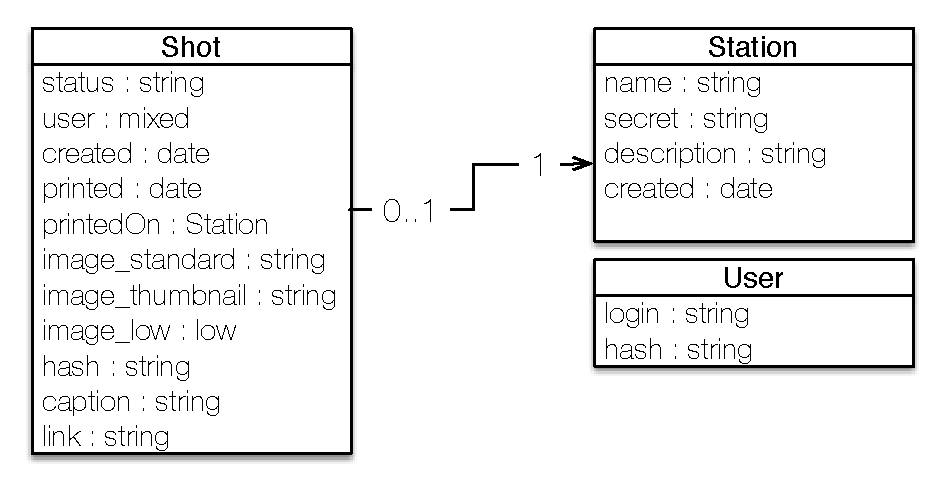
\includegraphics[scale=0.8]{data-model-uml.pdf}
    \caption{схема базы данных}
    \label{fig:DataModel}
\end{center}
\end{figure}

Модель \texttt{User} служит для хранения данных об администраторах системы, которые могут управлять очередью посредством
веб-интерфейса.

\subsection{Обработчики запросов от веб-интерфейса}
Предоставление прикладного интерфейса по протоколу HTTP реализовано с помощью библиотек Express.js~\cite{ExpressJS} и
Passport.js~\cite{PassportJS}. Express.js представляет собой легковесный серверный веб-фреймворк, а Passport.js служит
для организации возможности авторизации.

\begin{figure}[htbp]
\begin{center}
  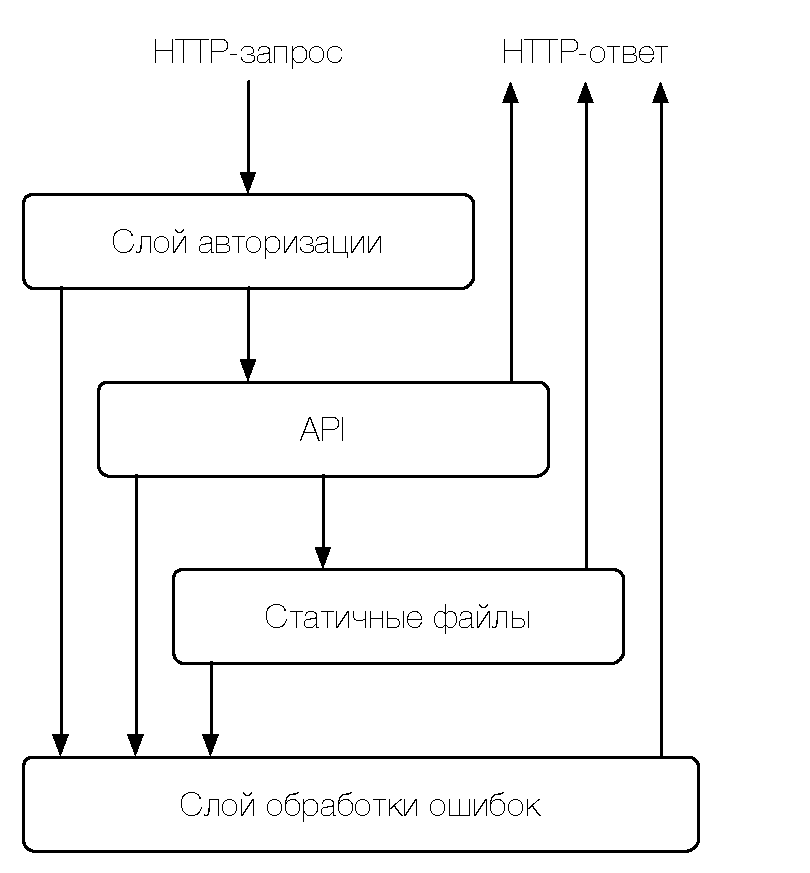
\includegraphics[scale=0.8]{http-routing.pdf}
    \caption{схема обработки HTTP-запросов в приложении}
    \label{fig:HttpRouting}
\end{center}
\end{figure}

Библиотека Express.js позволяет строить сложные веб-приложения на основе маршрутизации HTTP-запросов через так называемые
промежуточные слои (англ. \textit{middleware}). Каждый слой может на основе определенных условий послать ответ на запрос,
а может пропустить запрос к следующему слою. Существуют слои, которые предоставляются самой библиотекой или
сторонними пакетами: слой авторизации, слой статических файлов, слой обработки параметров форм и т.~д. Кроме того,
библиотека позволяет программисту определять собственные слои, которые работают на основе соответствия URL-адреса определенному
шаблону (шаблоном может быть строка или регулярное выражение). Таким образом, веб-приложение представляет собой граф
промежуточных слоев, благодаря чему возможно построение гибких веб-приложений с понятной архитектурой.

Рассмотрим архитектуру промежуточных слоев, используемую в приложении (рис. \ref{fig:HttpRouting}). Слой авторизации
необходим для определения пользователя, который в данный момент работает с системой (информация о пользователе хранится
в модели \texttt{User}). Данный слой предоставляется библиотекой Passport.js и отвечает за обработку хранимых в
Cookie сессий. Далее следует слой API, предоставляющий прикладные функции для работы с моделями. Наконец, слой статичных
файлов служит для отдачи файлов клиентского веб-интерфейса. Любые ошибки, возникающие в слоях, перенаправляются в слой
обработки ошибок (под ошибками подразумеваются ошибки времени выполнения, например, необработанные исключения).

Слой API реализует обработчики для управления моделями \texttt{Station} и \texttt{Shot} в соответствии с парадигмой
REST. Это означает, что модели интерпретируются как ресурсы веб-сервера, над которыми можно выполнять действия (читать,
создавать, удалять и обновлять), используя определенные соглашения о формировании запросов.

Рассмотрим методы, предоставляемые API для работы с ресурсом \texttt{Stations} (печатные станции):

\begin{description}
  \item[\texttt{POST /stations}] \hfill\\Регистрация новой печатной станции в системе. Данный метод требует права администратора.
  \item[\texttt{GET /stations}] \hfill\\Получение списка печатных станций, зарегистрированных в системе.
  \item[\texttt{GET /stations/:id}] \hfill\\Получение информации о конкретной печатной станции по идентификатору.
  \item[\texttt{PUT /stations/:id}] \hfill\\Изменение полей печатной станции: описания, названия и ключа. Данный метод требует
    права администратора.
  \item[\texttt{DELETE /stations/:id}] \hfill\\Удаление печатной станции по идентификатору. Данный метод требует права
    администратора.
\end{description}

Рассмотрим методы, предоставляемые API для работы с ресурсом \texttt{Shots} (фотография): %Точно ShotS?

\begin{description}
  \item[\texttt{GET /shots}] \hfill\\Получение списка всех фотографий. Данный метод поддерживает: сортировку, фильтрацию по
    статусу и печатной станции и ограничение количества фотографий для показа (для организации
    постраничной загрузки). Параметры фильтров являются частью адреса, например запрос \texttt{GET /shots?limit=5\&status=failed}
    вернет пять последних фотографий, которые не были напечатаны в результате ошибки.

  \item[\texttt{GET /shots/:id}] \hfill\\Получение информации о конкретной фотографии по идентификатору.
  \item[\texttt{DELETE /shots/:id}] \hfill\\Удаление фотографии по идентификатору. Данный метод требует права
    администратора.
  \item[\texttt{GET /shots/:id/queue}] \hfill\\Помещение заданной фотографии в очередь печати. Данный метод требует права
    администратора.
\end{description}

Кроме того, API предоставляет следующие методы для авторизации:
\begin{description}
  \item[\texttt{POST /auth/login}] \hfill\\Метод, используемый для авторизации в системе. В случае успешной авторизации создается
    сессия, которая сохраняется между запросами с помощью Cookie.

  \item[\texttt{POST /auth/logout}] \hfill\\Метод, используемый для очистки текущей сессии (выхода из системы).

  \item[\texttt{GET /auth}] \hfill\\Данный метод возвращает информацию о текущей сессии. Он используется веб-приложением для
    проверки прав доступа.
\end{description}

Большая часть описанных методов использует формат JSON для формирования ответа. Ответ может содержать информацию о
запрашиваемой сущности, а также дополнительную мета-информацию. Например, метод \texttt{GET /shots}, который может
возвращать часть списка всех фотографий для экономии трафика и организации постраничного вывода, также включает в результат
мета-информацию о количестве всех фотографий с системе (рис.~\ref{fig:JsonResponse}).

\begin{figure}[t!]
\begin{center}
  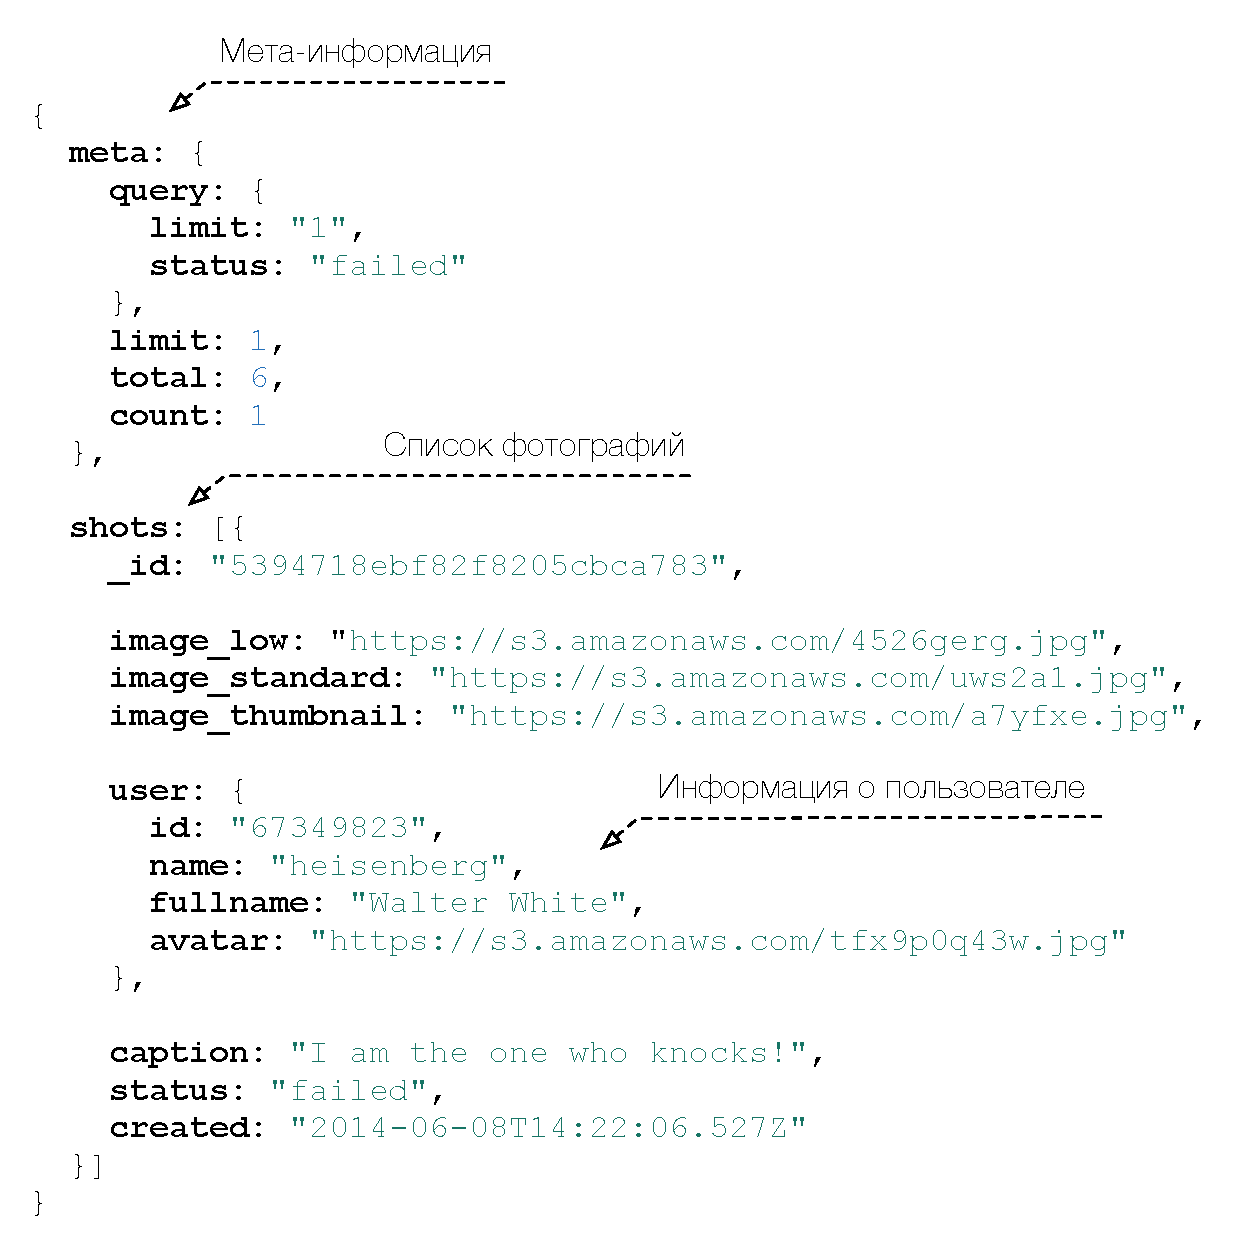
\includegraphics[scale=0.7]{json-response.pdf}
    \caption{пример ответа от сервера при вызове метода \texttt{GET /shots}}
    \label{fig:JsonResponse}
\end{center}
\end{figure}


\subsection{Веб-интерфейс и синхронизация моделей}
Веб-интерфейс для управления заданиями печати представляет собой одностраничное веб-приложение, которое использует
клиентский веб-фреймворк Chaplin~\cite{ChaplinJS}.

В основе приложения лежит паттерн проектирования MVC, подразумевающий использование следующих компонентов:
\begin{itemize}
  \item \textbf{Роутер} --- обработчик глобального состояния приложения, в задачи которого входит осуществление перехода между
    страницами.
  \item \textbf{Модели} --- локальное (на стороне веб-браузера) представление моделей, хранящихся в базе данных.
  \item \textbf{Вид} --- отображение моделей на странице, которое изменяется при изменении атрибутов моделей.
  \item \textbf{Контроллер} --- компонент, отвечающий за подгрузку данных с сервера и обеспечение связи между моделью и видом.
\end{itemize}

При разработки данного интерфейса была использована система сборки Brunch~\cite{Brunch}, которая позволила:

\begin{enumerate}
  \item Организовать компиляцию организованных в модули скриптов на CoffeeScript в один минифицированный JavaScript файл.
    Был использован модульный подход к организации файлов в соответствии со спецификацией CommonJS~\cite{CommonJS}.

  \item Использовать для описания элементов интерфейса препроцессор стилей Stylus~\cite{Stylus} и шаблонный язык
  Jade~\cite{JadeLang}. Язык Jade предназначен для формирования шаблонов, на основе которых во время выполнения
  генерируются части страницы. Препроцессор Stylus расширяет возможности каскадных таблицей стилей (CSS), позволяя
  использовать так называемые <<примеси>> и обеспечивая поддержку нестандартизированных свойств во всех современных
  браузерах.

  \item Обеспечить поддержку автоматической перезагрузки страницы (технология LiveReload) при сохранении исходных файлов.
  Применение такого подхода позволило сделать процесс разработки максимально прозрачным и гибким.
\end{enumerate}

Описываемое приложение имеет следующие состояния:
\begin{itemize}
  \item Форма авторизации.

  \item Список печатных станций.
     \begin{itemize}
        \item Страница конкретной печатной станции с описанием.
        \item Страница редактирования станции.
     \end{itemize}

  \item Галерея фотографий, содержащая напечатанные и находящиеся в печати фотографии.
\end{itemize}

\begin{figure}[t!]
\begin{center}
  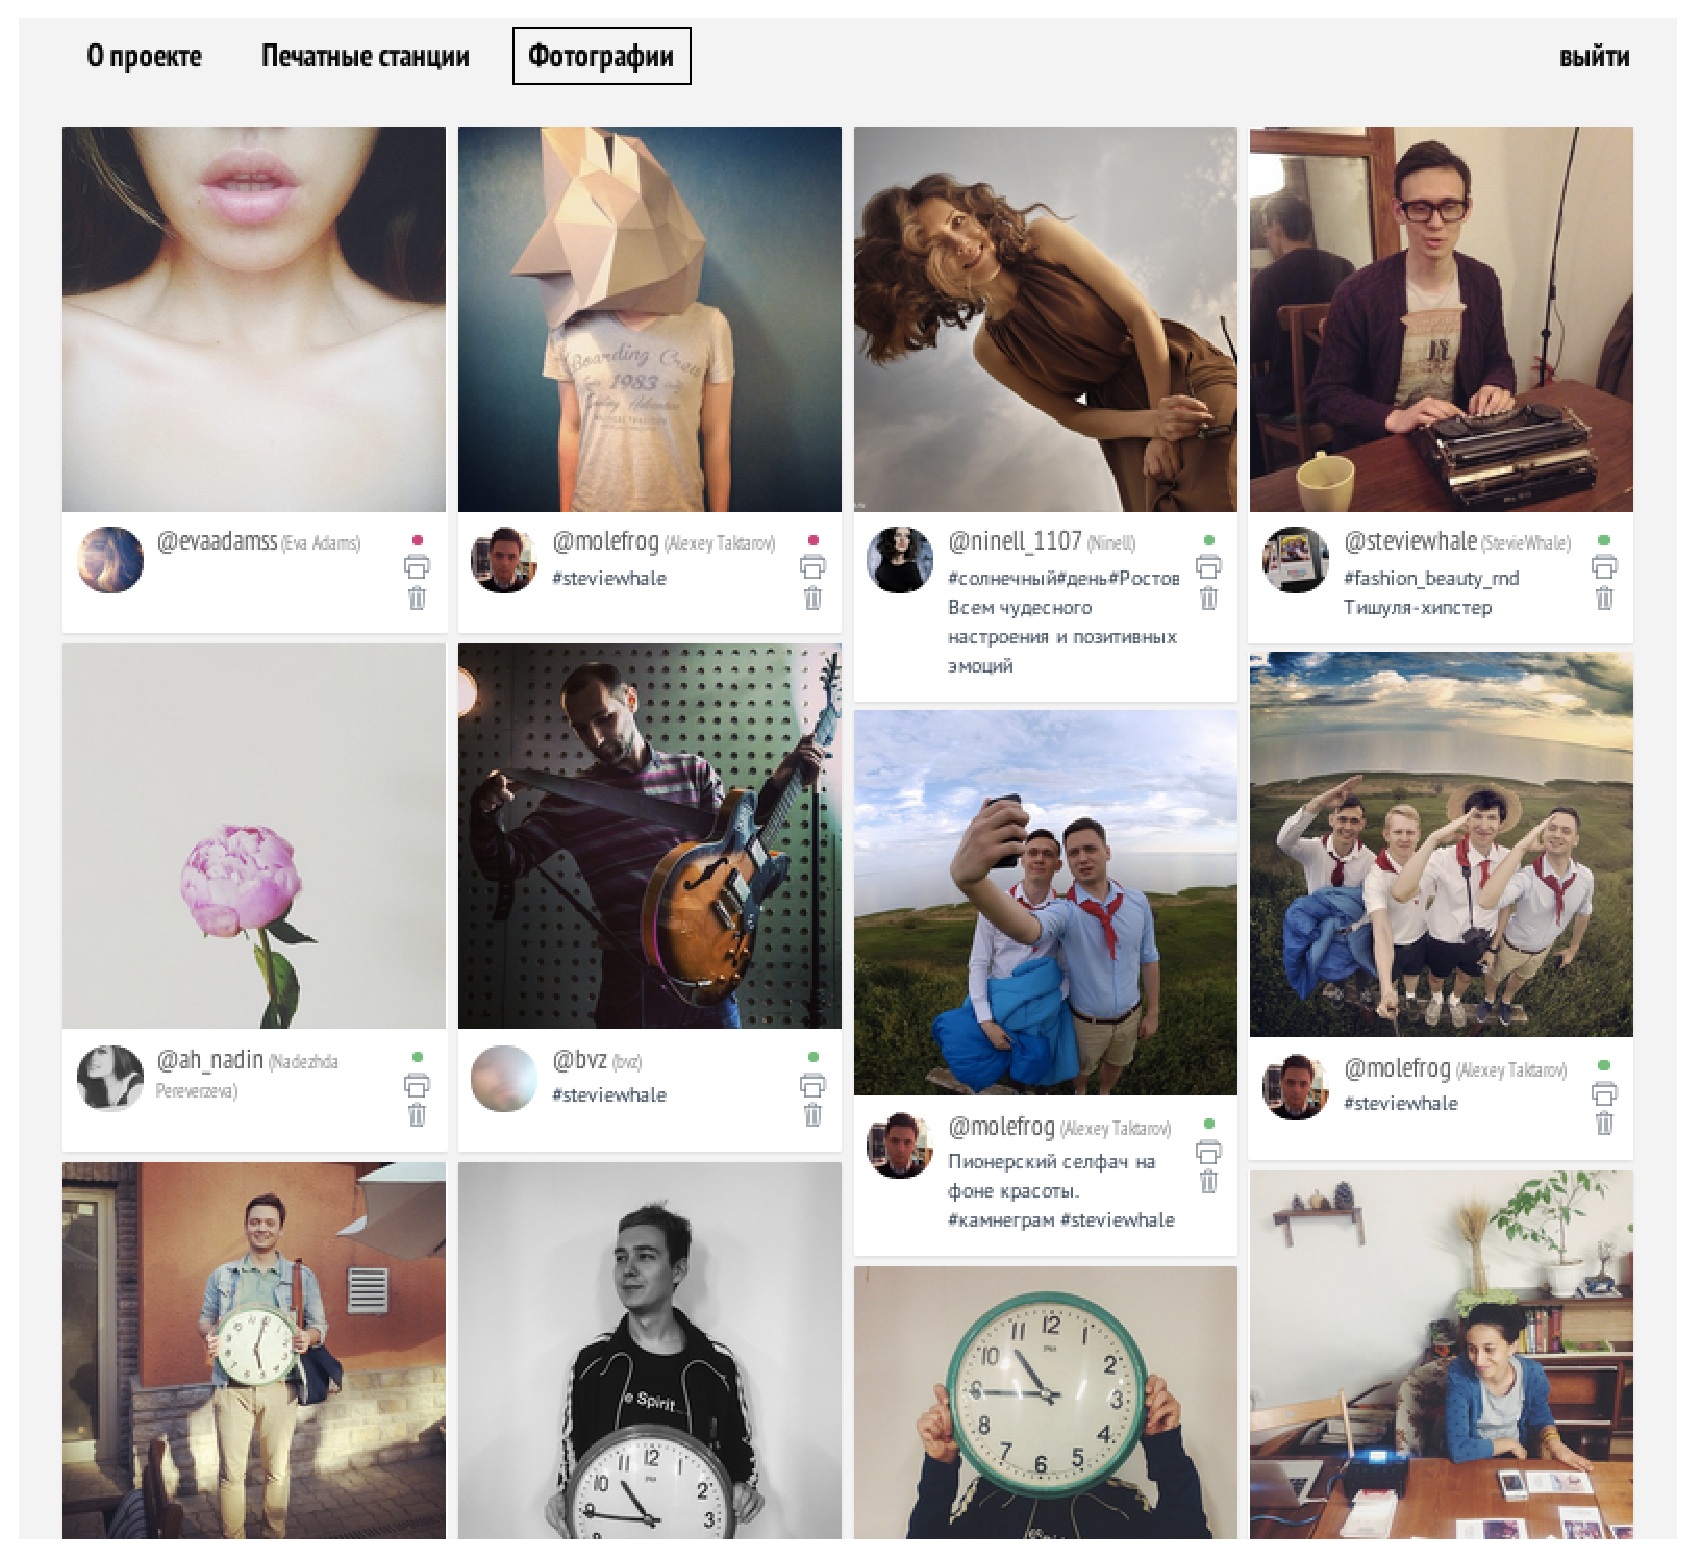
\includegraphics[scale=0.53]{grid-interface.pdf}
    \caption{интерфейс галереи фотографий}
    \label{fig:GridInterface}
\end{center}
\end{figure}

Центральным компонентом является галерея фотографий (рис. \ref{fig:GridInterface}), которая одновременно служит
архивов напечатанных фотографий и средством мониторинга процесса печати в режиме реального времени. Для компоновки
фотографий в виде сетки была использована библиотека Masonry~\cite{Masonry}. Одним из требований при реализации
этого компонента была возможность моментального получения уведомлений об изменении фотографий на сервере.
Подобная синхронизация моделей была достигнута благодаря использованию транспорта, который предоставляется библиотекой
socket.io~\cite{SocketIO}.

Изменение модели фотографии на сервере может привести к рассылке всем подключенным через веб-интерфейс клиентам
следующих сообщений:
\begin{itemize}
  \item \texttt{shot.updated}, когда статус фотографии был изменен (например, фотография перешла из статуса <<в очереди>>
  в статус <<напечатана>>);
  \item \texttt{shot.created}, когда новая фотография была добавлена в очередь печати;
  \item \texttt{shot.removed}, когда фотография была удалена.
\end{itemize}

Обработка серверных событий синхронизации происходит через глобальный объект \textbf{Медиатор}~\cite{MediatorPattern}.
Данный компонент принимает уведомления, поступающие от сервера посредством канала socket.io. Отдельные части интерфейса
(в данном случае вид галереи фотографий) подписываются на события, которые генерирует Медиатор, и производят
соответствующие обновления отображения. Применение такого подхода позволило снизить зависимость частей приложения друг
от друга и добиться максимальной гибкости при разработке.

\subsection{Очередь печати фотографий}
Распределение задач печати между подключенными к системе агентами осуществляется посредством глобальной очереди печати,
функционирующей в рамках центрального сервера. Очередь является незаменимым средством при проектировании многокомпонентных
систем, в которых происходит распределение вычислений среди нескольких узлов. Кроме того, использование очередей позволяет
реализовать следующие схемы взаимодействия: очередь заданий (англ. \textit{work queue}), отправка сообщений
подписчикам~\cite{RabbitMQ} (англ. \textit{publish/subscribe}) и удаленный вызов про\-це\-дур~\cite{DistributiveSystems}.


\begin{figure}[htbp]
\begin{center}
  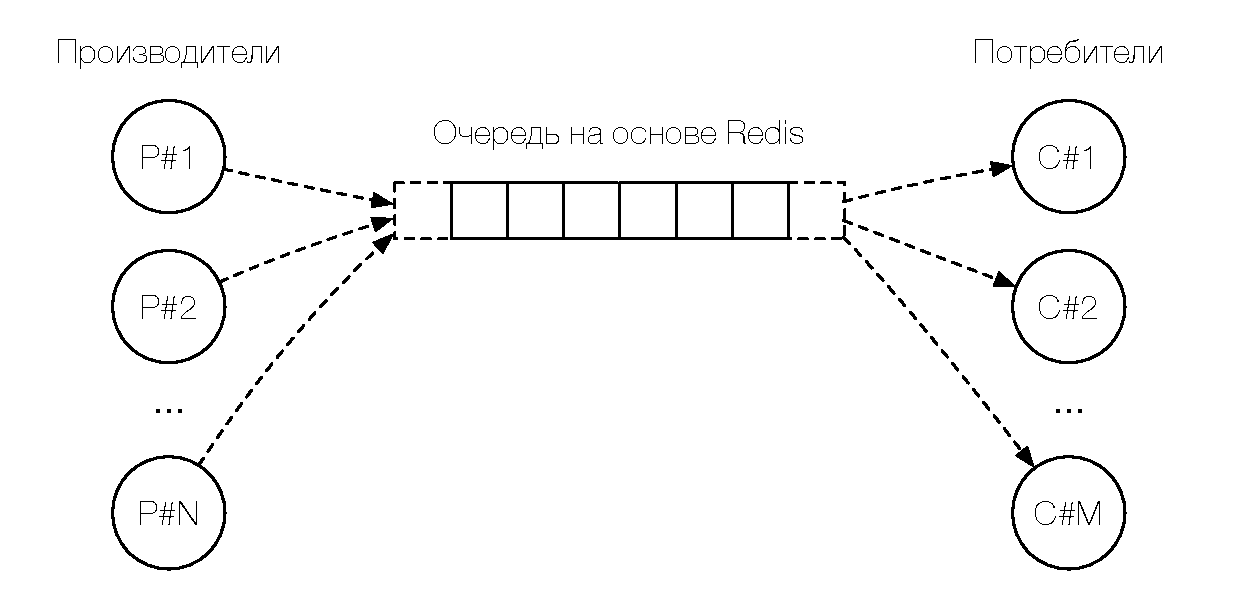
\includegraphics[scale=0.8]{producer-consumer.pdf}
    \caption{схема работы очереди <<производитель-потребитель>>}
    \label{fig:ProducerConsumer}
\end{center}
\end{figure}


В описываемой системе была использована очередь заданий, реализованная при помощи библиотеки Kue~\cite{Kue} и базы данных
Redis. Данная очередь работает по принципу <<производитель-потребитель>>. Компоненты приложения, называемые
\textbf{производителями}, генерируют задания и помещают их в очередь, к которой имеют доступ \textbf{потребители},
извлекающие задания и исполняющие их (рис. \ref{fig:ProducerConsumer}). Использование хранилища Redis позволяет
сохранять информацию о заданиях после перезапуска центрального сервера, кроме того применение данной схемы приводит к
возможности разбиения приложения на несколько независимых процессов, каждый из которых выполняет заданную функцию
(создает задания или исполняет их).

Опишем последовательно реализацию компонентов центрального сервера, взаимодействующих с очередью печати.

\subsubsection{Модуль поиска фотографий в социальной сети}
Новые фотографии для печати поступают в систему при помощи публикации в социальной сети Instagram. Однако необходим
способ, который бы позволил отделить фотографии для печати от общего потока фотографий в сервисе. Это может быть
достигнуто при помощи добавлении специальной метки к описанию фотографии --- \textit{хештега}.

\begin{figure}[t!]
\begin{center}
  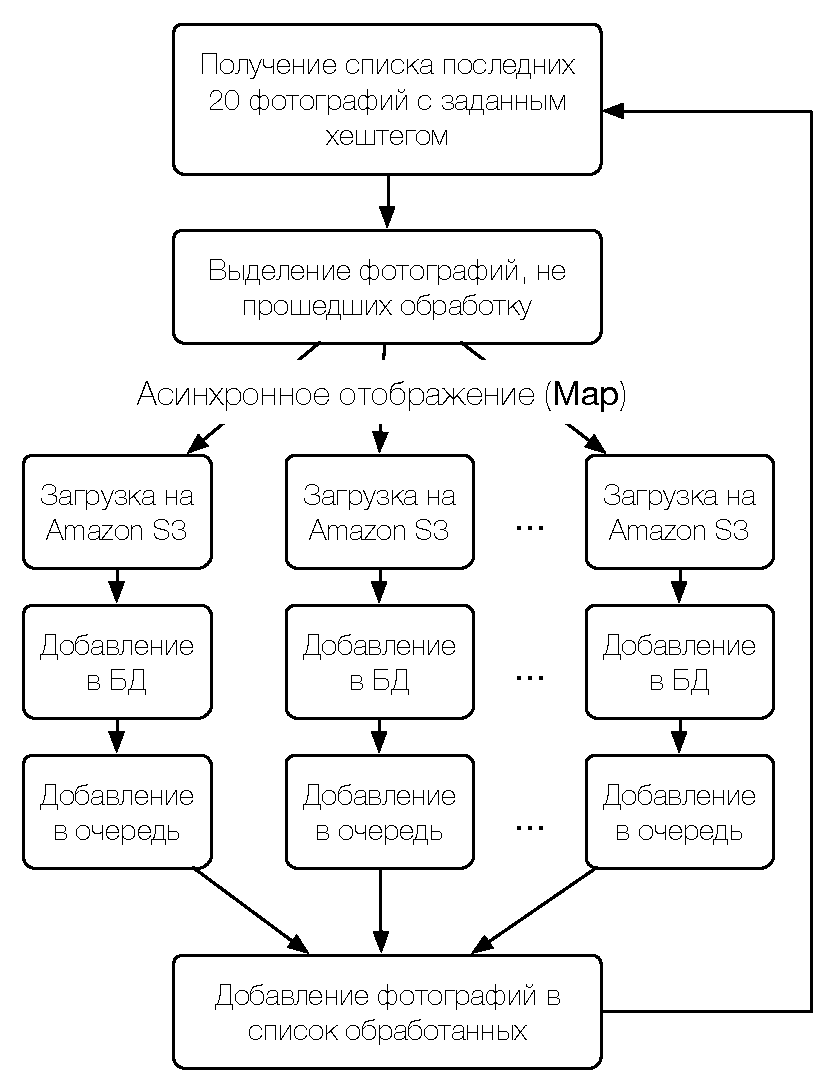
\includegraphics[scale=0.8]{map-reduce.pdf}
    \caption{схема работы модуля поиска фотографий}
    \label{fig:MapReduce}
\end{center}
\end{figure}

В рамках описываемой системы реализован модуль поиска новых фотографий в социальной сети, которые содержат заданный
хештег. Для этого были использованы возможности публичного API сервиса Instagram. Принцип работы данного модуля заключается
в периодическом опросе сервиса на предмет наличия новых фотографий с указанным хештегом.

Сервис Instagram предоставляет функцию \texttt{tags.recent}, возвращающую 20 последних записей, помеченных заданным
хештегом. Полученная порция фотографий фильтруется модулем для выделения тех фотографий, которые еще не прошли обработку.
Далее, список новых фотографий с помощью асинхронного паттерна Map (отображение), реализованного в библиотеке
Async~\cite{Async}, проходит обработку (рис. \ref{fig:MapReduce}). Прежде всего, происходит загрузка изображений в
облачное хранилище файлов Amazon S3 (для того, чтобы избежать потери данных в результате удаления фотографии в социальной сети),
затем создаются записи в базе данных (используется модель \texttt{Shot}). Наконец, идентификаторы созданных записей помещаются
в очередь печати.

\subsubsection{Обработка заданий печати}
Опишем алгоритм обработки заданий печати, поступивших в очередь:
\begin{description}
  \item \textbf{Шаг 1.} Загрузить из базы данных соответствующую данному идентификатору модель \texttt{Shot}.
  \item \textbf{Шаг 2.} Выбрать доступную печатную станцию из списка подключенных. При отсутствии станций пометить
    данную фотографию как ненапечатанную.
  \item \textbf{Шаг 3.} Сформировать на основе данных о фотографии изображение для печати.
  \item \textbf{Шаг 4.} Загрузить сформированное изображение в облачное хранилище файлов Amazon S3.
  \item \textbf{Шаг 5.} Вызвать удаленную процедуру \texttt{print} на выбранной печатной станции, передав в качестве
    параметра ссылку на сформированное изображение.
  \item \textbf{Шаг 6.} После завершения печати удалить изображение из хранилища и обновить статус фотографии в базе
    данных.
\end{description}

\begin{figure}[t!]
\begin{center}
  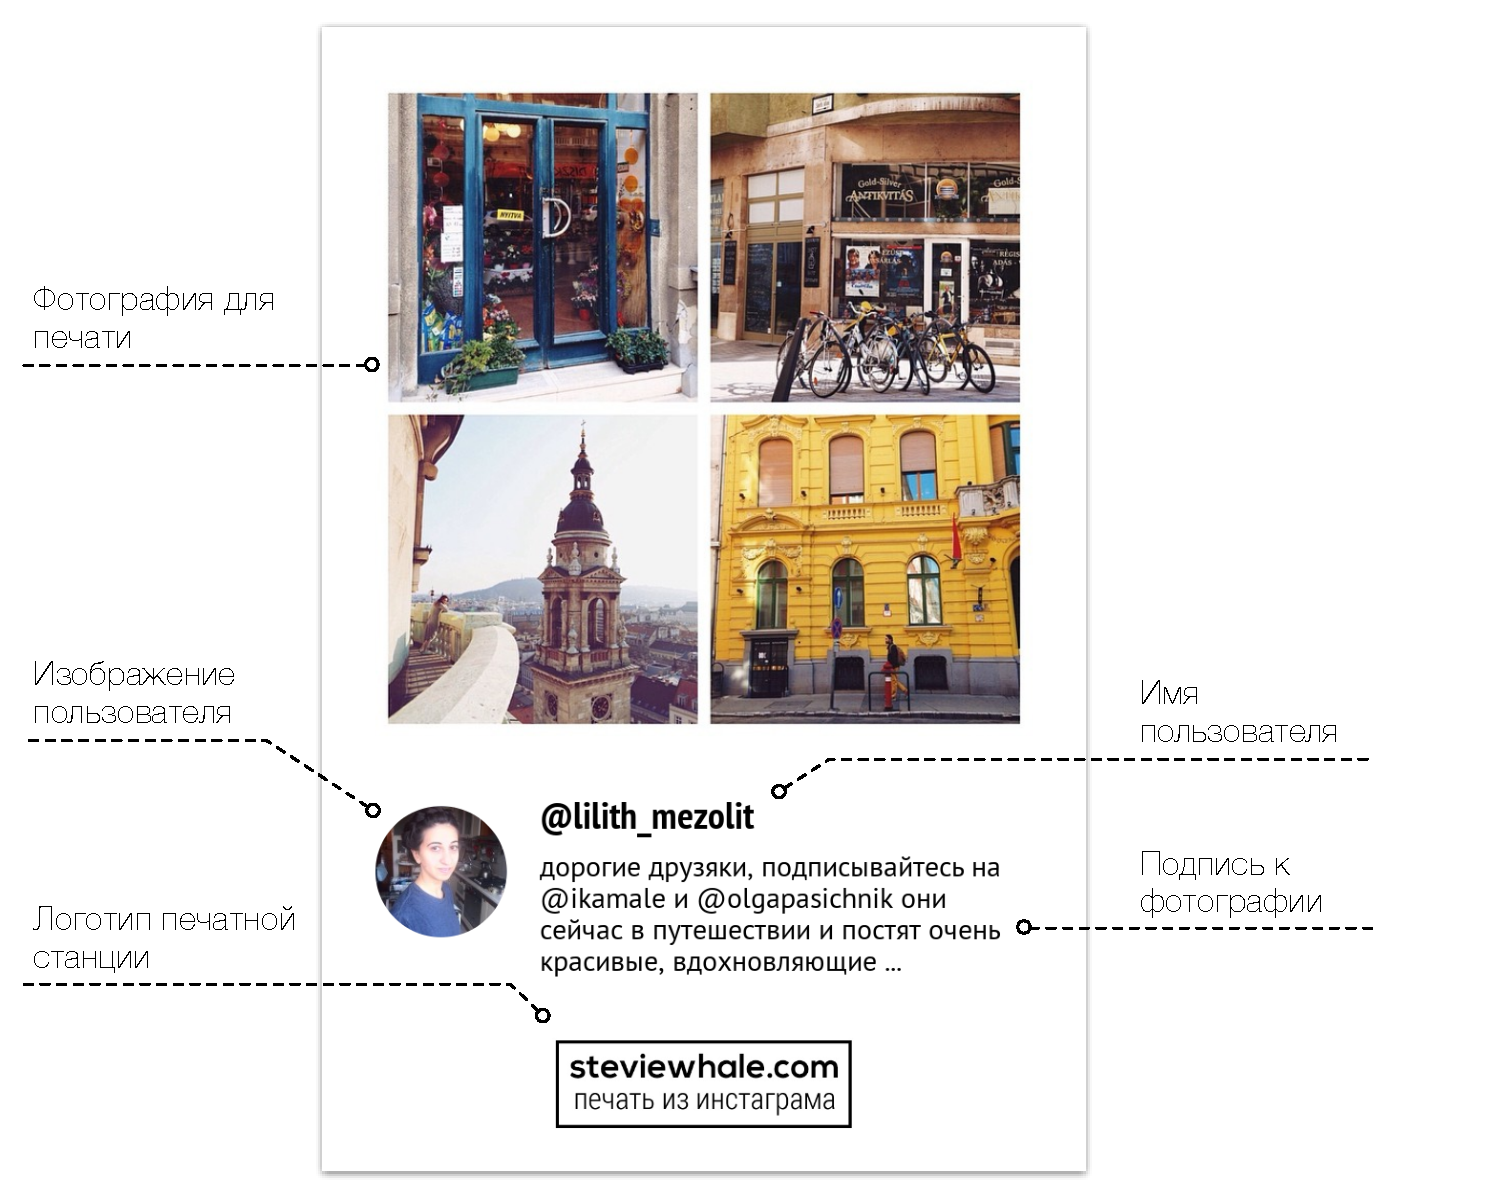
\includegraphics[scale=0.65]{photo-layout.pdf}
    \caption{пример сформированного для печати изображения}
    \label{fig:PhotoLayout}
\end{center}
\end{figure}

Печатаемое изображение содержит помимо самой фотографии также информацию о пользователе, опубликовавшем запись
в социальной сети (рис. \ref{fig:PhotoLayout}). Для формирования данного изображения используется библиотека node-canvas,
реализующая методы объекта Canvas из HTML5  для Node.js. Отличительной особенностью такого решения является
возможность прямой загрузки результирующего изображения в облачное хранилище, минуя файловую систему (с использованием
потоков ввода-вывода).

\section{Интеграция}
Разработка больших систем зачастую сопряжена с трудностями запуска работающей версии продукта в производство. 
Обычно причинами являются
 сложность развертывания компонентов, недостаточная стабильность работы системы и несоответствие окружения, в
котором происходит разработка, среде, предполагающей долгую работу приложения.

В данной главе описываются решения, с помощью которых были решены приведенные проблемы в рамках разработанного
комплекса. За основу был взят принцип <<12-факторного приложения>>~\cite{TwelveFactor}, представляющий собой методологию
построения поддерживаемых и масштабируемых облачных сервисов.

% Про что хочется:
%   + окружения и конфиги
%   + тесты и непрерывная интеграция
%   + логи в облако
%   + деплой
%   + запуск на Raspberry Pi

\subsection{Разделение окружений}

\subsection{Тестирование и непрерывная интеграция}

\subsection{Процедура развертывания}
В рамках разработанной системы был реализован процесс автоматического развертывания при сохранении кода в удаленный
репозиторий. Это возможно благодаря событиям системы контроля версий Git и скрипту на языке Bash, выполняющему необходимую
для запуска новой версии программы подготовку~\cite{PushDeploy}.

Опишем шаги, которые входят в процедуру развертывания:
\begin{description}
  \item \textbf{Шаг 1.} Остановить работающую версию приложения.
  \item \textbf{Шаг 2.} Установить необходимые для веб-интерфейса и серверной части зависимости посредством пакетных
    менеджеров NPM и Bower.
  \item \textbf{Шаг 3.} Выполнить сборку статичных файлов веб-интерфейса.
  \item \textbf{Шаг 4.} Запустить обновленную версию приложения.
\end{description}

\newpage
\section*{Заключение}
\addcontentsline{toc}{section}{Заключение}


\newpage
\addcontentsline{toc}{section}{Список литературы}

\bibliographystyle{unsrt}
\bibliography{bibliography/sources}

\end{document}
